% -----------------------------------------------------------------------------
% Trabalhos Relacionados
% -----------------------------------------------------------------------------

\chapter{Trabalhos Relacionados}
\label{chap:trabRelac}

Neste capítulo são discutidos trabalhos que foram tomados como base para a construção do presente projeto. Levando em consideração que o tema abordado está sendo discutido e aplicado na indústria de tecnologia, foram selecionados quatro trabalhos para análise, sendo um deles com viés acadêmico e os outros três com viés de mercado. 

A primeira parte do capítulo é focada em apresentar a dissertação de mestrado de Miika Ruissalo \cite{ruissalo2018operating}, que trata-se de um estudo de viabilidade de implementação de \textit{design system} em uma grande empresa de tecnologia e telecomunicações finlandesa. Em seguida, são apresentados três casos de implementações do \textit{design system} em empresas consolidadas no mercado: Ryte, Gusto e Airbnb. Em cada um dos casos, foram destacadas as motivações e aprendizados adquiridos durante o processo de implementação.

Finaliza-se o capítulo com uma breve discussão a respeito das semelhanças identificadas entre os diferentes trabalhos.

\section{Dissertação de mestrado de Miika Ruissalo}
\label{sec:teseMestrado}

Ao se investigar a ocorrência de trabalhos relacionados na literatura, aquele que apresentou maior similidaridade, no que se diz respeito ao seu propósito, foi a dissertação de mestrado de \citeonline{ruissalo2018operating}.

Intitulada \textit{Operating a design system in a large software company}, \citeonline{ruissalo2018operating} discute o fenômeno \textit{design system} como proposta de solução para problemas de consistência e escalabilidade que empresas de tecnologia acabam vivenciando durante o fluxo de desenvolvimento de seus produtos em larga escala. A fase empírica do projeto se demonstrou como um estudo da aplicação da metodologia por uma grande empresa de tecnologia e telecomunicações finlandesa. A empresa em questão havia passado por um processo de restruturação do seu design, criando seu próprio \textit{design system}. Tal evento ocorreu três anos antes do desenvolvimento da dissertação.

O experimento teve duração de seis meses, período ao qual foram observados sete dos vários times de desenvolvimento de produtos da empresa. O grupo amostral escolhido para o experimento foi cuidadosamente selecionado para garantir que todos os contextos chave da organização seriam cobertos pela pesquisa. O \autoref{table:ruissaloTeams} apresenta as características de cada um dos times selecionados.

\begin{quadro}
  \centering
  \begin{tabular}{|m{2cm}|m{4cm}|m{8cm}|} \hline
    
    \multicolumn{1}{|c|}{\bfseries Time} & \multicolumn{1}{c|}{\bfseries Contexto e Plataforma} & \multicolumn{1}{c|}{\bfseries Considerações importante} \\\hline
    
     Time 1 & B2B - Web & Um designer do time criou parte considerável dos \textit{assets} \footnote{O termo \textit{Asset} é normalmente utilizado para referenciar atributos como imagens, \textit{scripts} e folhas de estilo, comumente presentes em sistemas web.} do sistema \\\hline
     
     Time 2 & Mercado consumidor - Web e Mobile & Começou a utilizar tecnologias relevantes recentemente, incluindo o \textit{design system} \\\hline
     
     Time 3 & Mercado consumidor - Web & Um dos três times que construiu a base de toda a plataforma \\\hline
     
     Time 4 & Ferramenta B2B - Web & Time surgiu pouco tempo antes da realização do experimento \\\hline
     
     Time 5 & Ferramenta B2B - Mobile & A criação do \textit{design system} não levou em consideração o contexto desse time \\\hline
     
     Time 6 & Mercado consumidor - Web & Trabalha com projetos de curta duração e que geram impacto rapidamente \\\hline
     
     Time 7 & Mercado consumidor - Plataforma específica & Não pode utilizar o \textit{design system} devido ao contexto da plataforma específica não o permitir \\\hline
     
      
  \end{tabular}
  \caption{Características dos times estudados por \citeonline{ruissalo2018operating}}
  \fonte{Adaptado de \citeonline{ruissalo2018operating}}
  \label{table:ruissaloTeams}
\end{quadro}

A metodologia adotada pela dissertação consistiu basicamente em duas grandes fases: observação e entrevistas. Na primeira fase, \citeonline{ruissalo2018operating} dedicou seu tempo a observar o dia-a-dia de cada um dos times selecionados, estando posicionado estratégicamente próximo de três destes. Na segunda fase, o pesquisador realizou entrevistas com dois grupos distintos de profissionais: designers e desenvolvedores. Cada grupo, portanto, experimentou um roteiro de entrevista diferente do outro.

Como resultado do experimento, foi observado que uma das maiores queixas dos profissionais de desenvolvimento de produto é a falta de uma fonte única da verdade. Esse foi um dos principais argumentos utilizado pelos times quando a empresa sob estudo optou por desenvolver seu \textit{design system}. A maioria dos benefícios apontados no \autoref{chap:fundamentacaoTeorica} do presente trabalho foi parceptível na empresa finlandesa, tanto na visão da organização quanto na visão dos designers e desenvolvedores. Consistência, poder de reusabilidade e velocidade no desenvolvimento foram características observadas no produto e nos times analisados pela dissertação, exemplificando assim a metodologia de \textit{design system} como um verdadeiro sucesso no desenvolvimento de produtos digitais em uma grande organização.

\section{Ryte}
\label{sec:ryte}

A Ryte é uma organização cujo produto principal oferece a capacidade de monitoramento, análise e otimização dos \textit{sites} de seus clientes de forma a garantir melhores taxas de desempenho. Ela conta atualmente com uma cartela de mais de 500.000 usuários ativos em sua plataforma.

Seu produto surgiu como resultado de uma repaginação do antigo \textit{OnPage.org}. No artigo \textit{Lessons learned building a Design System for 500,000+ users at Ryte} \cite{ryteDesignSystem}, o autor discute os desafios que surgiram como consequência dessa transição.

O artigo tem início com \citeonline{ryteDesignSystem} afirmando que, nos momentos iniciais da transição, toda a equipe estava bastante motivada. Por esse motivo, a plataforma ganhou forma com bastante velocidade, porém sem consistência alguma. Os diversos times que compunham a organização trabalhavam isoladamente uns dos outros, produzindo assim diferentes soluções para um mesmo problema. Com quatro meses de projeto, percebeu-se que o caminho que estava sendo traçado não era sustentável e que medidas deveriam ser tomadas imediatamente.

Naquele momento, a empresa enfrentava três grandes problemas que deveriam ser solucionados o quanto antes. O primeiro deles era o fato de que todos os produtos da plataforma eram muito diferentes uns dos outros, tanto visualmente quanto em relação à experiência do usuário ao utilizá-los. Com 11 tipos distintos de \textit{pop-ups}, 23 tipos de botões e 67 tons de cinza diferentes, os usuários acabavam tendo que reaprender os mesmos conceitos quando utilizavam uma nova ferramenta disponibilizada pela plataforma. O segundo problema era um pouco mais grave: um processo de design lento e ineficiente. O tempo para se construir novas funcionalidades era elevado, uma vez que era preciso reconstruir a grande maioria dos componentes presentes na entrega do zero. Por fim, o último ponto a ser resolvido era a falta de identidade de marca no mercado. Além de inconsistências na plataforma, não havia correlação alguma entre os mecanismos de marketing e a plataforma em si.

Inspirada em empresas como Shopify, Atlassian e Hubspot, a Ryte buscou na metodologia do \textit{design system} uma solução para os seus problemas. A abordagem utilizada consistia basicamente em dois componentes: um arquivo Sketch \footnote{O Sketch é uma ferramenta de design gráfico voltada para prototipação de interfaces de usuário
desenvolvida pela Bohemian BV, e é disponibilizada em <https://www.sketchapp.com/>.} e um repositório Git \footnote{O Git é um sistema de controle de versões distribuído. Normalmente é usado no desenvolvimento de software, mas pode ser utilizado para registrar o histórico de edições de qualquer tipo de arquivo.} compartilhados. Não foram abordados fatores como tom de voz e princípios de design nessa primeira versão. Além disso, não existe interligação clara entre artefatos de design e artefatos de desenvolvimento e a justificativa para tal decisão reside no fato de que o time identificou problemas de escalabilidade ao se unir os dois mundos.

Como resultado imediato da implementação do \textit{design system} percebeu-se: processo de design oito vezes mais rápido, mais velocidade no desenvolvimento de novas funcionalidades e um maior poder de escalabilidade. \citeonline{ryteDesignSystem} ainda compartilha no artigo alguns dos aprendizados que o time vivenciou ao longo do processo. Tais aprendizados são consolidados e apresentados no \autoref{table:ryteLessonsLearned}.

\begin{quadro}
  \centering
  \begin{tabular}{|m{4cm}|m{10cm}|} \hline
    
    \multicolumn{1}{|c|}{\bfseries Aprendizado} & \multicolumn{1}{c|}{\bfseries Comentário} \\\hline
    
     Não reinventar a roda & Existem várias bibliotecas de componentes prontas no mercado que podem ser utilizadas como base. \\\hline
     
     A biblioteca de componentes é um documento vivo & Ao se desenvolver novas funcionalidades, constantemente surgem novos componentes a serem incluidos na biblioteca. Deve-se evitar ao máximo incluir novos componentes semelhantes a algum já existente. Nesses casos, é preferível dar manutenção a este. \\\hline
     
     Aproximar o produto dos mecanismos de marketing & Podem existir problemas durante essa unificação -- como diferentes tamanhos de fonte, por exemplo --, porém isso é necessário. \\\hline
     
     Envolver pessoas chave no processo & Certificar-se de que existem pessoas com um bom \textit{background} técnico para a tomada de decisões importantes. Também é importante envolver pessoas com diferentes contextos no processo. \\\hline
     
     Comunicação com o desenvolvedor é fundamental & Transmitir a importância do \textit{design system} para o desenvolvedor é fundamental, pois só assim haverá a garantia de que as decisões tomadas pela metodologia serão refletidas no produto. \\\hline
      
  \end{tabular}
  \caption{Aprendizados da implementação do \textit{design system} da Ryte.}
  \fonte{Adaptado de \citeonline{ryteDesignSystem}}
  \label{table:ryteLessonsLearned}
\end{quadro}

\section{Gusto}
\label{sec:gusto}

A Gusto é uma empresa que facilita o gerenciamento de folhas de pagamento e benefícios dos funcionários de seus clientes. Fundada em 2011, atualmente conta com cerca de 60.000 clientes ativos em sua plataforma.

Foi iniciado, em 2016, um projeto de criação de um \textit{design system} para a organização. No artigo \textit{Design Systems at Gusto: Part I}, escrito por Robin Rendle \cite{gustoDesignSystem}, é apresentado todo o processo de desenvolvimento do mesmo.

Problemas nos processos de design e desenvolvimento eram as principais motivações para a criação do \textit{design system}. Na época, o time de produto da empresa era composto por nove designers de produto e muitos engenheiros de desenvolvimento. Gerir uma comunicação eficaz entre os diferentes times e profissionais envolvidos na plataforma era um grande desafio que, até então, não havia sido solucionado. Não existia, ainda, nenhuma biblioteca de componentes que guiasse a tomada de decisão de design dos times. Como consequência, a base de código-fonte \textit{frontend} da plataforma se tornou muito grande e confusa, o que impactava diretamente a capacidade de escalabilidade do produto.

Foi nesse momento que Rendle decidiu, de maneira proativa, iniciar os trabalhos de construção do novo \textit{design system} da Gusto. Durante esse processo foram acumulados alguns aprendizados, que foram consolidados no \autoref{table:gustoLessonsLearned}.

\begin{quadro}
\centering
\begin{tabular}{|m{4cm}|m{10cm}|} \hline
	
	\multicolumn{1}{|c|}{\bfseries Aprendizado} & \multicolumn{1}{c|}{\bfseries Comentário} \\\hline
	
	 É impossível construir um \textit{design system} sozinho & A pior coisa que se pode fazer para uma empresa é se provar como sendo o seu colaborador mais inteligente. Esse tipo de postura gera desconforto por parte dos outros membros da empresa e negligencia pontos de vista diferentes do seu. \\\hline
	 
	 Um \textit{design system} não precisa estar completo para ser útil & Como seu propósito é sanar os problemas de toda uma organização, a nível de design de produto, é comum se empregar muito esforço para a construção de um \textit{design system} perfeito. A verdade é que, por mais simples que ele seja, um \textit{design system} por si só já gera um valor muito grande, uma vez que ele centraliza as tomadas de decisões de design de produto da empresa. \\\hline
	 
	 \textit{Design Systems} surgem e morrem por conta de sua documentação & A documentação de um componente é tão importante quanto o componente em si. Caso a maneira como um componente deve ser manipulado não seja auto-explicativa, seus usuários tenderão a evitá-lo. \\\hline
	 
	 Um \textit{design system} é um repositório de conhecimento & \textit{Design Systems} não são importantes somente por representar precisamente a base de código, mas também por diminuir a complexidade social de uma organização, estimulando a comunicação e concentrando o conhecimento. \\\hline
    
\end{tabular}
\caption{Aprendizados da implementação do \textit{design system} da Gusto}
\fonte{Adaptado de \citeonline{gustoDesignSystem}}
\label{table:gustoLessonsLearned}
\end{quadro}

Rendle finaliza seu artigo destacando uma das vantagens de se implementar um \textit{design system}: garantir que a comunicação entre todos os membros envolvidos no produto ocorra de maneira fluida e de acordo com as diretrizes de design e produto da organização. Na \autoref{fig:socialComplexityIncrease}, o autor ilustra a maneira como a complexidade de comunicação dentro de uma empresa aumenta consideravelmente conforme novos talentos são incluídos no processo. Reintara, ainda, o papel fundamental de um \textit{design system} como facilitador da comunicação entre os times.

\begin{figure}
	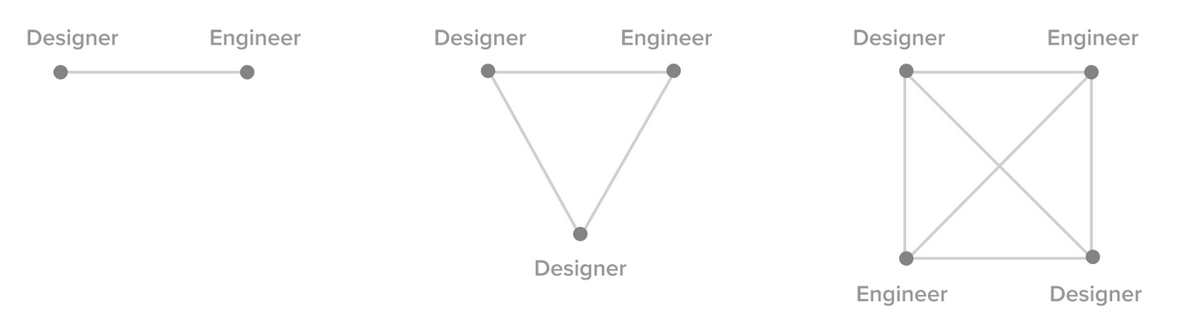
\includegraphics[width=\linewidth]{./04-figuras/03_trabalhos_relacionados/social-complexity.png}
    \caption{Evolução da complexidade social de uma empresa}
    \fonte{\citeonline{gustoDesignSystem}}
    \label{fig:socialComplexityIncrease}
\end{figure}

\section{Airbnb}
\label{sec:airbnb}

Como último exemplo de trabalho relacionado ao presente documento, será apresentado o estudo de caso de implementação do \textit{design system} da Airbnb. Com sede em San Francisco - California, Estados Unidos, a Airbnb é uma famosa empresa que opera um mercado online global de serviços de hospedagem acessível através de seu site e aplicativo para dispositivos móveis.

No artigo \textit{Building a Visual Language}, produzido por \citeonline{airbnbDesignSystem} e disponibilizado diretamente no site oficial da empresa, discorre-se sobre a trajetória de criação do sistema, poderando-se suas motivações e aprendizados adquiridos ao longo do processo.

Devido ao seu crescimento acelerado, problemas de escalabilidade do produto surgiram rapidamente, conforme a empresa conquistava maiores parcelas do seu mercado e aumentava o tamanho de sua equipe de desenvolvimento.

O primeiro problema apresentado foi a falta de padrões disseminados entre as equipes. Esse fator contribuia para a criação de uma variedade de artefatos que resolvem o mesmo problema, muitas vezes ocasionando em experiências de usuários distintas ao longo de toda a plataforma.

Em seguida, o artigo menciona o problema de se ter múltiplos designers e \textit{stakeholders} trabalhando em uma mesma plataforma. A maior dificuldade, nesse ponto, seria manter consistência em todo o produto.

Outro fator motivador para a criação do \textit{design system} foi a necessidade de se dar suporte a múltiplas plataformas e dispositivos. Sem uma biblioteca de componentes flexível, o fenômeno do retrabalho acaba sendo inevitável. Uma mesma funcionalidade deveria ser implementada várias vezes, dependendo da quantidade de plataformas que a empresa suportasse.

Para sanar os problemas citados, a Airbnb decidiu por construir o seu próprio \textit{design system}. O processo de criação foi exaustivo, porém o resultado final foi um sucesso. Dos exemplos citados no presente trabalho, o \textit{design system} da Airbnb é, sem dúvidas, o mais completo. Nele, além da biblioteca de componentes, também foram trabalhados os artefatos de princípios de design e tom de voz. Por isso, o trabalho realizado pela Airbnb é hoje uma das referências do mercado no que se diz respeito a \textit{design systems}.

\citeonline{airbnbDesignSystem} também compartilha alguns dos aprendizados adquiridos pela sua equipe no artigo. Tais aprendizados foram consolidados no \autoref{table:airbnbLessonsLearned}.

\begin{quadro}
\centering
\begin{tabular}{|m{4cm}|m{10cm}|} \hline

	\multicolumn{1}{|c|}{\bfseries Aprendizado} & \multicolumn{1}{c|}{\bfseries Comentário} \\\hline
	
	 Nem todos os componentes são criados igualmente & Alguns componentes podem ter variações de implementações para diferentes plataformas. Em alguns casos, manter essa segregação é mais saudável e facilita a manutenção. \\\hline
	 
	 Documentação & A atividade de documentação dos componentes deve fazer parte do processo de criação, independentemente dos prazos de entrega. A falta de documentação dos componentes pode gerar muita confusão. \\\hline
    
\end{tabular}
\caption{Aprendizados da implementação do \textit{design system} da Airbnb}
\fonte{Adaptado de \cite{airbnbDesignSystem}}
\label{table:airbnbLessonsLearned}
\end{quadro}

Pode-se perceber, principalmente pelos depoimentos apresentados nas Seções \ref{sec:ryte}, \ref{sec:gusto} e \ref{sec:airbnb}, que as motivações que levam empresas a adotarem o \textit{design system} internamente são muito semelhantes. A dificuldade de se manter consistência no produto, a baixa velocidade de desenvolvimento e a falta de um repositório único que concentre as decisões de design são problemas comuns em empresas de tecnologia. Nesse contexto, o \textit{design system} vem se mostrando uma solução bastante eficaz.

No capítulo seguinte é apresentada a metodologia empregada pelo presente projeto para validar a eficácia de se utilizar um \textit{design system}, sob o ponto de vista de um desenvolvedor.
